\chapter{Implementation}
\label{chap:imp}
\lhead{\emph{Project Implementation}}
%This chapter should comprise 15 pages and enumerate your experience when doing what you wanted to do the way you wanted to do it.
The implementation of the system has changed drastically since the original plan due to an oversight where it was believed that the Pistache framework could handle the functionality for both the API and the synchronisation between the tree parity machines. The project turned out to be much more involved and difficult than originally expected. This means that the original sprint plan is no longer representative of the actual sprint plan used. This is however to be expected in an agile environment where the following sprint is normally determined after the evaluation of a sprint that was just completed. Despite all of this the system is functional and produces the same outcome as intended.

\section{Difficulties Encountered}
%Enumerate the different difficulties you have found when developing your solution approach. Create three categories of difficulties:
%\begin{itemize}
%    \item \textbf{Easy}: You managed to solve the problem with little difficulty.
%    \item \textbf{Medium}: It was not easy to solve, but you managed to develop a workaround or solution and %still achieve the functionality you originally had in mind.
%    \item \textbf{Hard}: The difficulty was so complicated that you didn’t managed to solve it. As a result, some functional requirement / non-functional requirement or use case from your solution approach was not achieved.
%\end{itemize}

%For each difficulty, classify it into easy, medium or hard. Then, provide the following info:
%\begin{enumerate}
%    \item Description of the difficulty: Brief description of the problem you found.
%    \item How did it affect the original project design?: Indicate how this difficulty affected:
%    \begin{enumerate}
%        \item the architecture of your solution
%        \item if it represented a risk to your project
%        \item if it affected your methodology to develop your project
%        \item if it changed your implementation schedule
%        \item if it changed the evaluation plan
%    \item What did you do to manage the difficulty arisen?: Brief description of your decision to overcome the %difficulty.
%    \end{enumerate}
%\end{enumerate}
The major difficulties I encountered were primarily related to the architecture of the project. The initial class diagrams were way too basic and didn't account for the fact that Pistache would now only be used for the API and nothing else. 

\textbf{Easy Difficulty}
\begin{enumerate}
\item The NodeJs module was replaced with simply a NodeJs App. The NodeJS module is not implemented due to a time constraint and is not necessary to the outcome of the project. The NodeJs module was originally meant to simplify the communication with the API for people who wish to use it. A NodeJS App would need to be implemented regardless in order to use that module and demonstrate the usability of the API. 
The API doesn't have many routes to use therefore it would not be difficult to use the API with any NodeJs App as interacting with the API is simply done with POST requests. The final NodeJs App that is in the same GitHub repository, consumes the API perfectly as well as purposely demonstrating some aspects of dynamic cryptography that would normally be hidden. Any user that wishes to use the API can simply copy the functions in the NodeJs App that interact with the API and change them accordingly to send and receive their own data. It is recommended for users to copy said functions as there are specific steps that need to take place to register the NodeJS App with the API in particular the synchronisation service. For this reason The NodeJs App uses pure NodeJs libraries like ExpressJs \cite{ExpressJS} which is the most popular routing framework for NodeJs. The NodeJs App has no front end as it would be difficult for users wishing to use the API to adapt the front end too, therefore only a basic HTML template engine is used to deal with the HTML. JavaScript for the front end is purely used for visual purposes and is not required since all of the information sent from the browser to the NodeJs app is done through classic HTML forms. This doesn't have any impact on the architecture as the NodeJS App is not really included in the architecture as it is simply designed to consume the API. This does impact the schedule in a positive way as it is easier and quicker to simply make a NodeJS App than a NodeJs module and a NodeJs App.
\end{enumerate}

\textbf{Medium Difficulty}
\begin{enumerate}
\item The sprints needed to be adjusted to accommodate the new implementation plan. The final sprint plan will be placed here as it briefly reflects the major changes that took place, these changes will be discussed in more detail in the following sections. The Sprint plan follows a two week sprint approach.
\begin{table}[h]
\centering
\caption{New Sprint Plan}
\begin{tabular}{|p{1cm}|p{12cm}|}
\hline Sprint & Tasks \\ [14pt]

\hline 1 & Create a basic API server that can process GET and POST requests. Familiarise self with RapidJSON library \cite{rapidjson} and create functions to parse C++ objects into JSON "strings" and JSON "strings" back into C++ objects. Research peer to peer libraries, no useful ones were found. Decided to make a custom one with the help of the Boost ASIO \cite{boost_asio_home} library. Never used Boost ASIO before therefore a decision was made to follow the developers tutorials on the Boost ASIO website. This was not enough to understand the complicated library therefore other tutorials such as this one \cite{boost_asio_totorial_1} were also followed.  \\ [12pt]

\hline 2 & Further knowledge of Boost ASIO needed to be acquired before it was possible to proceed with coding the actual peer to peer network. Thankfully a very informative book called Boost.Asio C++ Network Programming \cite{boost_book} by John Torjo was purchased and ended up being the last resource needed in order to complete the peer to peer network. A basic peer to peer network was written however was unstable at the end of this sprint \\ [12pt]

\hline 3 & Peer to peer network works as expected. Implemented basic synchronisation with real tree parity machines. Implemented command line parsing using Boost Program Options \cite{boost_asio_cmd} to enable different options such as selective outputs and port configurations. Completed synchronisation between tree parity machines fully therefore they produce the same weights successfully. Implemented "logging" to external terminal windows. \\ [12pt]

\hline 4 & Research how to proceed with the API i.e have two separate processes or contain the API and peer to peer network within the same process. Decision was made to contain both in the same process for security reasons. Basic API server was constructed and could be easily spawned along side the peer to peer service.\\ [12pt]

\hline 5 & Implement API functionality for synchronisation. Changes needed to be made to the peer to peer service to accommodate unexpected requirements needed to begin synchronisation when using the API. AES encryption decryption implemented using Crypto++ \cite{cryptopp} library. Encrypted data needed to be encoded using base64 again with the help of Crypto++ library. Implement a NodeJs app to consume and demonstrate various features of the API.\\ [12pt]

\hline 5 & Test the system. Implement options to choose which parts of the system to log since logging everything at once can be difficult to demonstrate different aspects of the system. Clean up the code. Document instructions on how to setup the system in the GitHub Readme file. \\ [12pt]

\hline
\end{tabular} \\
\label{tab:ProjRisks}
\end{table}

\FloatBarrier


\item The API and the synchronisation could not be done using only the Pistache framework as originally believed. This was a fairly significant set back since I have experimented before with Pistache framework and was familiar with how it operated functionality wise. It was only until I attempted to use Pistache for synchronisation I discovered that my original plan will not work since Pistache is a very good REST framework and not much else. To synchronise the tree parity machines a peer to peer network seemed most appropriate in how the synchronisation was envisioned to take place. After searching for easy to use libraries that supported peer to peer networks nothing that matched the requirements was found. This lead to the conclusion that a custom peer to peer network would have to be built from scratch. The attention grew towards Boost Asio as it is the most flexible generic networking library for C++. Unfortunately this library is quite extensive and is not as abstract as some of the previous peer to peer libraries encountered. Since with Boost Asio you will still deal with sockets however this will allow for greater control provided you know how the library works and Boost Asio has excellent asynchronous support which is essential for a responsive server. It took almost two full sprints to learn how the library works which set my initial schedule back as it was planned to spend time to learn the new technologies that would be used however it was not expected to spend so much time learning said new technologies. However some of the lost time was made back since the design of the peer to peer network was simple and efficient which allowed for a large number of synchronisation requests to take place per second resulting in generating a valid key in around one second which satisfies the requirement and no further optimisations needed to take place. This occurrence changed the architecture significantly since originally this wasn't meant to be present. Overall I'm glad that this happened as I had a chance to learn one of C++'s most popular networking library. Another benefit of using Boost Asio for synchronisation over Pistache apart from the fact that its impossible to achieve using Pistache is because the Boost Asio library is a lot lighter the performance increase is rather large. Obviously this would be impossible to test fairly however based on Pistache stress tests it can manage roughly 300 - 400 requests per second. The peer to peer Boost Asio can process around one thousand requests per second as it takes around one thousand requests for the tree parity machines to synchronise and they synchronise generally once per second.

\end{enumerate}


\textbf{Hard Difficulty}
\begin{enumerate}
\item A major difficulty that has prevented the implementation of a non functional requirement was the ability to use multiple tree parity machines per peer. Originally the plan was to implement multiple tree parity machines per peer, however in practice after spending more than a week on the problem a decision was made to move on and only allow one tree parity machine per peer. This theoretically does not have any impact on performance and certainly has no impact on security. A single tree parity machine per communication works as expected, a peer can have multiple tree parity machines where for example peer1 communicates with peer2 and peer3 at the same time. In this scenario peer1 would have two tree parity machines as the peer will communicate with two other peers. This scenario works flawlessly in the final implementation of the project. If the original plan were to be implemented peer1 would have twenty tree parity machines, ten per peer it communicates to. The reason why this is difficult is because the ten tree parity machines are reading and writing to the same socket. Whereas with one tree parity machine it has exclusive read and write access to the socket. An attempt was made to implement multiple read and write buffers, a queue, custom read and write objects however a decision was made to abandon this feature for now as it took up too much time and didn't add anything beneficial to the project apart from "being cool". 
The architecture of the project can be said to have changed although it is insignificant as the number of tree parity machines is rather virtual in nature. This issue did not represent any major risk to the project as everything works perfectly with one tree parity machine per connection. The implementation schedule was affected as a lot of time was spent on a feature that did not get implemented and it is better to spend time on features that actually do get implemented.
\end{enumerate}



\section{Actual Solution Approach}
%In December of last year, when writing the first version of the report, in Chapter 4 you came up with your original solution approach. On it, you presented (i) the architecture of your solution, (ii) your list of use cases, (iii) a risk assessment, (iv) a methodology to develop your solution approach, (v) your implementation schedule, (vi) your evaluation plan and (vii) some prototype of the resulting product. From January to April you have been developing your solution approach. Along the way you have encountered difficulties (the ones listed in Section 5.1) which might have modified your original plan so that you can come up with an actual developed project.
%This section is effectively the production of "as built" specification where you compare your original design to the final finished project. Please go section by section (the ones listed from (i) to (vii) in the last paragraph. For each section, enumerate any difference between the original design and the final project, and justify the difficulty forcing you to make such this change. Do not fret if some of these changes are radical, what is important here is that there is a clear rationale for changes made.
Most parts of my original approach to this project have changed vastly in particular the architecture. Every major change will be explored in the following sub sections.

\textbf{Architecture}

\begin{figure}[!h]
  \centering
      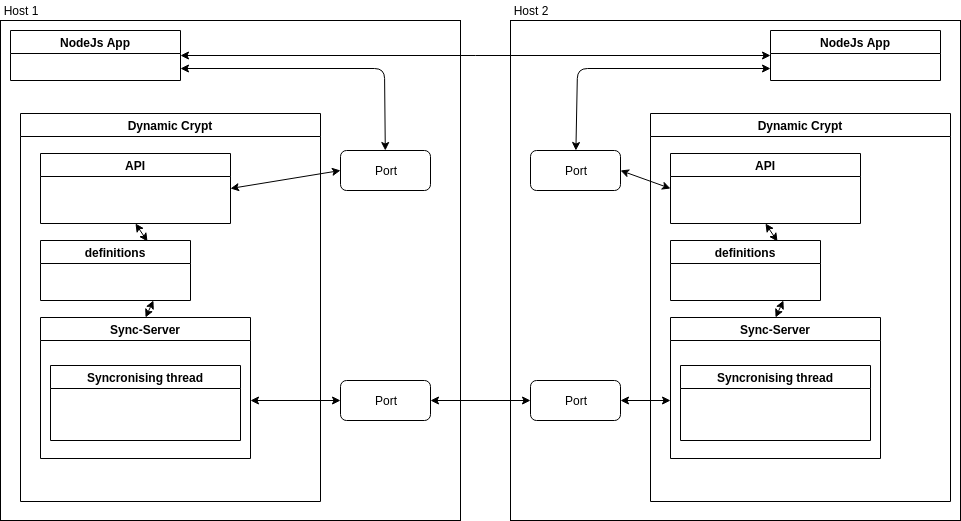
\includegraphics[width=1\textwidth]{Figures/basic-2hosts-final.png}
  \caption[High level overview of architecture]{High level overview of architecture}
  \label{fig:basic-two-hosts-final}
\end{figure}
\FloatBarrier

The high level overview of the architecture changed slightly as shown in figure \ref{fig:basic-two-hosts-final}. The functionality remains identical as described in the previous chapters. Initially the API and the server handling the synchronisation of tree parity machines executed in the same sort of architecture where the API would spawn threads for each tree parity machine. For the final implementation the API and the sync-server are separated into two servers. These two servers execute in the same process but obviously run on different threads. It was impossible to accomplish the task by using the API server alone as initially believed. This is because Pistache is limited to only API type operations as it is at its core built to code API rest applications. 

In order to be able to synchronise with any computer in the world the sync-server needed to be of a peer to peer nature. How this all works and why it is necessary will be explained in more detail later in chapter 6. Initially the API would spawn the tree parity machines due to the introduction of a new system this is still partially true however in the final implementation the API has access to a global function defined inside definitions.cpp that creates an instance of a peer object and connects to another listening peer. When the DynamiCrypt app executes an API instance is created and an instance of a listening peer is also created. This way the listening peer can accept any incoming connection and when an incoming connection arrives another peer is created and listens for more connections this way it is possible to theoretically have as many peers as possible synchronising provided the hardware supports it. 

By default the API is setup to use two threads this allows for multiple asynchronous requests to the API to be made with minimal wait time. The sync-server has a more much more heavy workload potential therefore by default it can use up to four threads. The sync-server by design is also asynchronous in operation therefore all of the four threads would most likely not be used at once. 

Initially there was not much of a consideration of how the API would communicate with the sync-server as it was overlooked since the system was vaguely defined at that point. However in the final implementation this is handled mostly through a global APIServiceDataHandler object that stores data relating to the NodeJs apps and contains the key store for each app "using" to the API.


\begin{figure}[!h]
  \centering
      \includegraphics[width=1\textwidth]{Figures/class-diagram-all-croped.png}
  \caption[DynamiCrypt Class Diagram]{DynamiCrypt Class Diagram}
  \label{fig:class-diagram-all}
\end{figure}
\FloatBarrier

Figure \ref{fig:class-diagram-all} represent the class diagram for DynamiCrypt as a whole. It is quite hard to make out the different elements since the class diagram is rather large therefore for the next sections this diagram will be split into mostly the API related classes and mostly sync-server related classes. This is here to briefly demonstrate how different classes interact with each other and how the the API interacts with the sync-server through mostly functions defined definitions. As you can tell this is nothing like the initial class diagram since to implement the system required a completely different solution that was not present in the initial plan.

\begin{figure}[!h]
  \centering
      \includegraphics[width=1\textwidth]{Figures/API_class_Diagram-croped.png}
  \caption[DynamiCrypt API Class Diagram]{DynamiCrypt API Class Diagram}
  \label{fig:API_class_Diagram}
\end{figure}
\FloatBarrier

Figure \ref{fig:API_class_Diagram} is a more clear and isolated representation of most of the classes used by the API. The APIServer is more of a wrapper class for APIservice as it sets up necessary Pistache objects required to use the Pistache REST framework and creates a fresh APIservice instance. 
The APIservice class itself is responsible for all the GET and POST routes available for the API and also deals with parsing JSON data as well as calling appropriate functions inside the API-service-data-handler object. 

The API-service-data-handler object is defined as a global object inside definitions.cpp as it needs to be accessed by both the sync-server when saving keys and the API when the API passes data for encryption and decryption as well as information about different services that want to use the API. For encryption and decryption the Crypto++ library is used, as well as for encoding and decoding to base64. The API-service-data-handler object has access to a key-store or sort of like an in memory only mini database that holds information about the services that are currently accessing the API and generated keys for said services, This is essentially a vector containing references to the APIdata object which in itself contains a vector of the keystore object. The API-service-data-handler object is called from within the APIservice when new services require the use of DynamiCrypt. The API-service-data-handler object also contains operations for custom dynamic encryption and decryption operations which will be discussed in detail later as it is quite interesting how they are designed. 

The definitions is a place that contains the applications global functions and variables such as defining the maximum size to use for the buffers, read and write locks for shared objects and other constants for defining which log messages to print. This also contains a vector of peers since by default there will be one peer listening for connections. The beginSync function creates a new peer which connects to a listening peer on another DynamiCrypt app. So each time a peer accepts a connection from another peer a new peer will be created to listen to more connections in its place and all of these peers will be added to this vector and can then be removed accordingly when a service decides to stop using DynamiCrypt. This occurs when the stopSync function is called which is called directly from the APIservice. Definitions also has a function for hashing strings as that is commonly used by the APIservice in the encrypt route.

The next two class diagrams \ref{fig:class_diagram_dynamicrypt-part1} and \ref{fig:class_diagram_dynamicrypt-part2} are both part of the sync-server classes so basically everything else that is not the API. However these are quite large therefore they are split into two separate diagrams. An attempt was made to make them look as continuous as possible where in the first diagram you can see relation lines going down of the page and continuing in the second diagram.

\begin{figure}[!h]
  \centering
      \includegraphics[width=1\textwidth]{Figures/class_diagram_dynamicrypt-part1.png}
  \caption[DynamiCrypt Class Diagram part 1]{DynamiCrypt Class Diagram part 1}
  \label{fig:class_diagram_dynamicrypt-part1}
\end{figure}
\FloatBarrier

Figure \ref{fig:class_diagram_dynamicrypt-part1} shows mostly the peer class and the TpmNetworkHandler class. The peer class contains the operations that read and write data to the socket and send it over to another peer. A more in dept explanation will follow in chapter 6 as to how data is read and written between peers. For now a basic explanation of the class will take place. The peer class uses Boost Asio to help with networking. The peer class implements interfaces such as enable shared from this and noncopyable as can be seen on the right hand side of the diagram.  Enable shared from this allows the peer object to be referenced by a smart pointer, which is handy when iterating through peers in a loop, a smart pointer is used because peer is an asynchronous class and if using a standard pointer there could be an issue with de-allocation of memory.  Noncopyable prevents objects of this class to be deep or shallow copied, this is mainly because this class has direct access to a socket and copying sockets is a really bad idea. Therefore peer objects should be only referenced by smart pointers and nothing else which noncopyable makes sure of.

As stated before peer is actually part of a peer to peer network hence the name however in this case the peer to peer network is very simple as it is a direct connection from one peer object to another, there is no such a thing as peer discovery or anything of that nature. In the thesis I mentioned listening peer and connecting peer multiple times. This is because how this object is initialised depends one the type of peer that is created. If initialising a peer in the following way. 

\begin{lstlisting}
ip::tcp::acceptor acceptor(service, ip::tcp::endpoint(ip::tcp::v4(), listen_port));
peer::ptr initial_peer = peer::new_(false);
acceptor.async_accept(initial_peer->sock(), 
    boost::bind(handle_accept,initial_peer,_1, &acceptor));
\end{lstlisting}
This peer will listen for other peers that connect to it. This is used exclusively in the main function after setting up the API server. 
And if initialising a peer in the following way.
\begin{lstlisting}
peer::ptr initiating_peer = peer::new_(true, address, port);
initiating_peer->start(service_name, partner_name);
\end{lstlisting}
This is a connecting peer which connects to the address and port specified in the parameters of its creation. The servicename and partnername are also passed in these are the details of the service that requested the use of DynamiCrypt through the API.

The rest of the functions deal with the different types of messages generated by each peer. Currently the messages are simple TCP data packets that indicate the type of message by simply by a number. More on this will be discussed in chapter 6.

The TpmNetworkHandler object exists for every peer and accompanied by a vector of SingleTpmNetworkHandler objects seen in figure \ref{fig:class_diagram_dynamicrypt-part2} takes care of the tree parity machines required for the peer. At the moment really only one tree parity machine is used for each connection between peers however provided I can fix the multiple buffer issue discussed earlier multiple tree parity machines could be used straight away for each peer. The TpmNetworkHandler object handles accessing, updating tree parity machines, generating input vectors, testing tree parity machines outputs as well as dealing with the more complicated TCP messages that were best left out from the peer class. The reason these were left out of the peer class is mostly because they are really long and require multiple accesses to tree parity machines therefore it is more efficient placing them inside TpmNetworkHandler where there is less references to go through. 

The SingleTpmNetworkHandler object in figure \ref{fig:class_diagram_dynamicrypt-part2} is quite similiar to the TpmNetworkHandler object in terms of some of its methods however it is only in charge of only one tree parity machine and therefore accesses it directly whereas the TpmNetworkHandler object would select the right tree parity machine to use and call methods found in the SingleTpmNetworkHandler object. The SingleTpmNetworkHandler object is also responsible for logging of important information about the tree parity machine it handles to an external terminal, such as how long it took to generate the key time wise and how many many synchronising iterations it took to to generate said key. 

The SystemHelper class provides a static method that helps to launch the external terminals. This class will be expanded in future versions of DynamiCrypt to allow for more OS specific functions such as running under its own user for more security. 

The TpmHandler, TPMInputVector, TreeParityMachine and DynamicArray classes are very similar to the original ones defined in the prototype. There are a few changes made to make them more secure but these can be considered unchanged from the original architecture.

Finally the definitions is here again it is blank this time as it was already discussed in figure \ref{fig:API_class_Diagram}. This time the peer sometimes uses the updatePeersChanged function in definitions when it disconnects and the SingleTpmNetworkHandler also uses definitions indirectly when adding the key to the keystore.

\begin{figure}[!h]
  \centering
      \includegraphics[width=1\textwidth]{Figures/class_diagram_dynamicrypt-part2-croped.png}
  \caption[DynamiCrypt Class Diagram part 2]{DynamiCrypt Class Diagram part 2}
  \label{fig:class_diagram_dynamicrypt-part2}
\end{figure}
\FloatBarrier

\begin{figure}[!h]
  \centering
      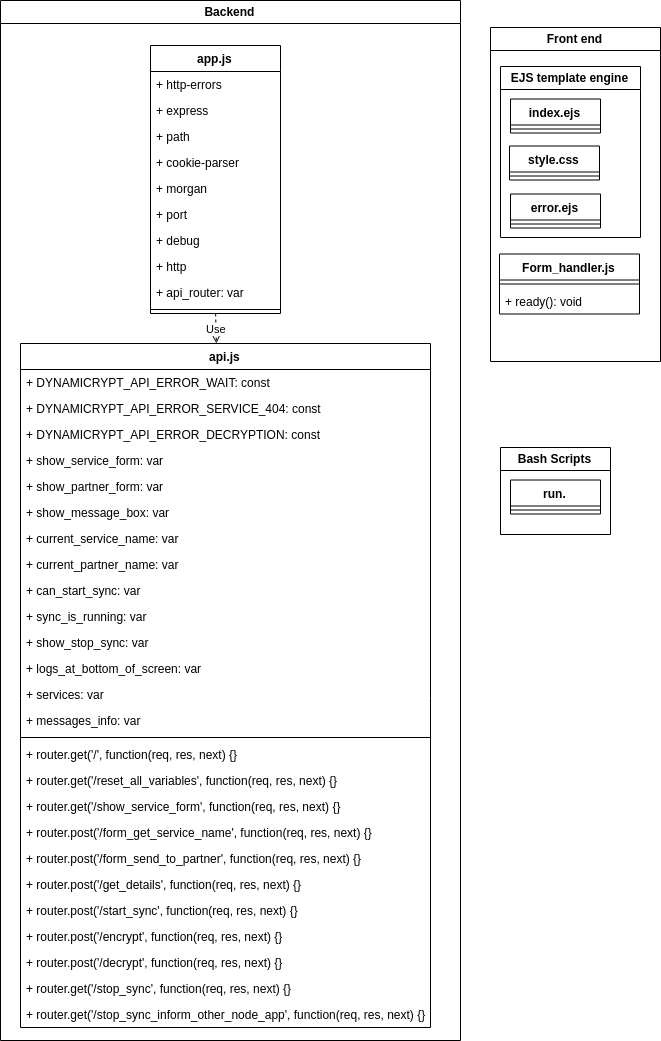
\includegraphics[width=1\textwidth]{Figures/nodeJsApp.png}
  \caption[NodeJs App architecture]{NodeJs App architecture}
  \label{fig:nodeJsApp_architecture}
\end{figure}
\FloatBarrier

The Final change in the architecture is the NodeJS app represented in figure \ref{fig:nodeJsApp_architecture}. Due to the nature of NodeJs in particular JavaScript you cannot really represent the language as a class diagram so I tried my best to represent the App as a whole and its major functions in a weird box diagram. Initially a NodeJs module would be made along side a NodeJS App however due to time constraints and a lot of time needed to be allocated for writing this thesis a decision was made to simple make a NodeJs app. 

The NodeJs app simply exists to consume and demonstrate the use of the API and the different modes of encryption / decryption supported by the API currently (more will be added in the next version). 

In order for other people to easily copy how the app interacts with the API every function that is related to the consumption of the API is located in the api.js file in the backend. For this reason no front end framework is used and the only interaction the backend has with the browser is through the forms submitted by the browser. It would be very easy to use something like ReactJS and provide a fluid front end that interacts with the DynamiCrypt API directly for some of the API calls however it would not be easy to copy and will confuse people trying to use DynamiCrypt API with their own custom Apps. In the future a better app demonstrating the API will be made that can be viewed as more of a real life app than something that demonstrates a technology will be made. But for now since only one app exists it is better to make it as clear as possible for people.

For parsing HTML EJS template engine is used which basically renders various forms depending on which Boolean variables are set, thereby making this NodeApp single paged. This also makes it easier for people to understand since all the routes are based on the root directory. and redirect to the root directory after each call so you will always see "/" in the browser. Since it a single page app only the index.ejs was required, by default webstorm also creates error.ejs however I have not touched this file. Finally there is a little bit of javascript using jquery however this is purely for visuals such as scrolling divs to the end and refreshing the page to make it seem more interactive, obviously if a front end framework were to be used this would not be required.

Lastly a bash script called run can be seen in the diagram this is just made so that it is easy to execute the NodeJs app on whichever port you want for example ./run 4000 will use port 4000 for the app, this is because to easily demonstrate the DynamiCrypt system it is better to have NodeJs apps running on multiple ports.
